\documentclass[10pt,twocolumn,letterpaper]{article}

\usepackage{cvpr}
\usepackage{times}
\usepackage{epsfig}
\usepackage{graphicx}
\usepackage{amsmath}
\usepackage{amssymb}
\usepackage{comment}
\usepackage[ruled,vlined,linesnumbered]{algorithm2e}
\usepackage{hyperref}
% Include other packages here, before hyperref.

% If you comment hyperref and then uncomment it, you should delete
% egpaper.aux before re-running latex.  (Or just hit 'q' on the first latex
% run, let it finish, and you should be clear).
\usepackage[breaklinks=true,bookmarks=false]{hyperref}

\cvprfinalcopy 

\def\cvprPaperID{****} 
\def\httilde{\mbox{\tt\raisebox{-.5ex}{\symbol{126}}}}

% Pages are numbered in submission mode, and unnumbered in camera-ready
%\ifcvprfinal\pagestyle{empty}\fi
\setcounter{page}{1}
\begin{document}

%%%%%%%%% TITLE
\title{Variational Autoencoders for Topic Modeling}
\author{Kelly Geyer\\
klgeyer@bu.edu}
\maketitle

%%%%%%%%% BODY TEXT
\section{Task}
%Describe the task you are going to solve, e.g. generating natural images like those shown in Fig. 1. Say a few words about what is difficult about the task, e.g. preserving spatial relationships, etc.
\noindent
Topic models are widely used for unsupervised learning of groupings, or topics, for a given corpus of documents. 
They are used in a variety of applications, which include language processing and bioinformatics. 
While there are several approaches to topic modeling, in this project we focus on improving the probabilistic topic models that assume the generative process of Latent Dirichlet Analysis (LDA), introduced by ~\cite{blei2012probabilistic}. 
In particular, this class of topic models uses Baysian modeling to estimate both the word-topic and document-topic probabilities. 
%In turn, these topic probabilities may be either visualized or clustered to summarize a large corpus of text. 
In recent works, probabilistic topic modeling has been improved in both performance and computational efficiency using VAEs ~\cite{miao2017discovering,srivastava2017autoencoding,burkhardt2019decoupling}. 

\paragraph{Objective.}
We want to explore potential improvements for topic modeling, using Variational Autoencoders (VAEs) ~\cite{kingma2013auto}. 
The authors of ~\cite{srivastava2017autoencoding} introduce two methods of VAE topic models, and compare them to traditional LDA.
Ultimately, we will replicate the analysis from ~\cite{srivastava2017autoencoding}.


%-------------------------------------------------------------------------

\section{Related Work}
%Describe 3-5 most related papers in detail, citing them in the following citation format, e.g.: Recurrent networks for image generation were proposed in [1]. Discuss potential flaws in these methods.
\noindent
In this project we compare the performance of three different types of topic models.
A topic model is an unsupervised method of clustering words into clusters, otherwise called \textit{topics}, as shown by Figure \ref{fig:concept}.
They take in a collection of documents, and return two types of summaries: (i) word-by-topic scores, and (ii) distributions over topics for each document.

\begin{figure*}
\begin{center}
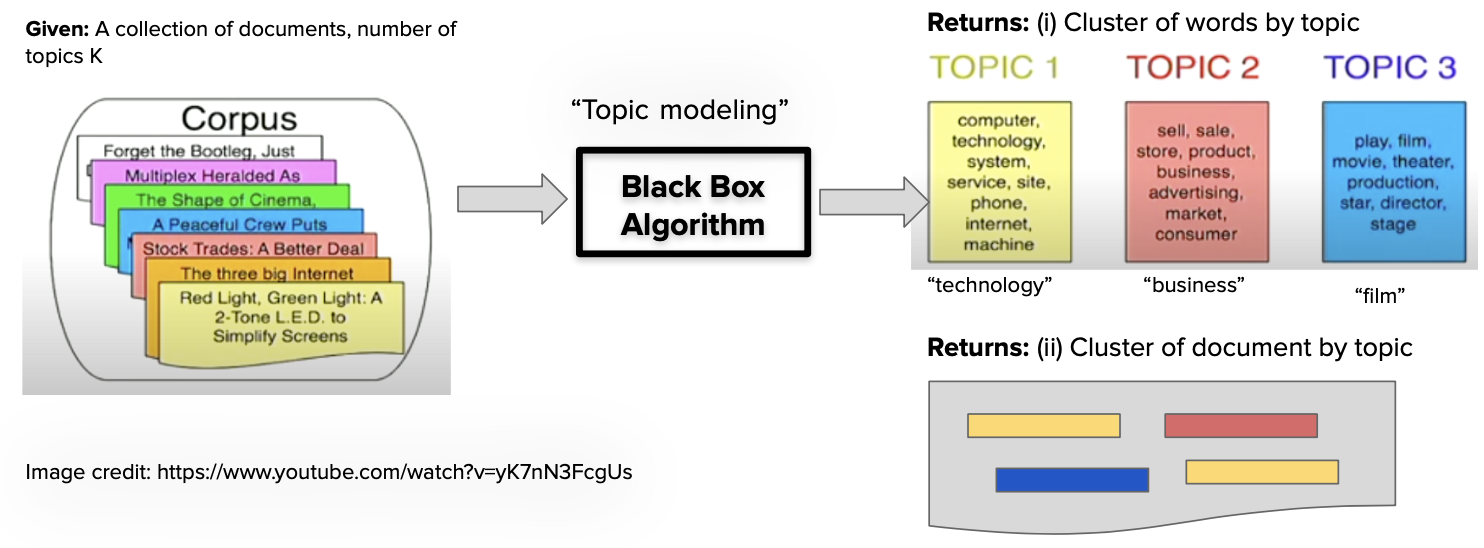
\includegraphics[width=1\linewidth]{topic-model-concept.png}
\end{center}
   \caption{Concept of a topic model: sort the words of a collection of documents into topics. They return (i) topic-by-word scores, and (ii) distributions for each topic over each document.}
\label{fig:concept}
\end{figure*}

\paragraph{Latent Dirichlet Analysis (LDA).} 
We consider generative topic models which assume that words, and respective their topics, are generated from a mixture probability distributions.
That is, the components of the mixture come from different \textit{topics}.
The original generative topic model, called Latent Dirichlet Analysis (LDA), was introduced by ~\cite{blei2012probabilistic}.
It assumes a generative process described by Algorithm \ref{alg:lda}.
Ultimately, LDA seeks to use Bayes' Theorem to estimate the parameters $\theta$ (document-topic scores) and $\beta_{z_n}$ (topic-document-word scores).
Overall, the marginal likelihood of a document $\bm{d}$ is 
\begin{equation}\label{eq:3}
    p(\bm{d}|\alpha,\beta) = \int_{\theta} \left(\prod_{n=1}^{N} \sum_{z_n=1}^{K} p(w_n|z_n,\beta) p(z_n|\theta)\right) p(\theta|\alpha)d\theta
\end{equation}
where $K$ is the number of topics.
\begin{algorithm}[t]\label{alg:lda}
\SetAlgoLined
 \For{each document $d = 1, 2, \ldots, D$}{
 Draw topic from distribution $\theta \sim \text{Dirichlet}(\alpha)$
 \For{each word in $d$, $w = 1, 2, \ldots, V$}{
 Sample topic $z_n \sim \text{Multinomial}(1, \theta)$ \\
 Sample word $w_n \sim \text{Multinomial}(1, \beta_{z_n})$
 }
 }
\caption{Generative process of LDA.}
\end{algorithm}

\paragraph{Autoencoded Variational Inference for Topic Models (AVITM).}
Applying a traditional Variational Autoencoder (VAE) to the LDA topic model formulation \eqref{eq:3} poses some some issues.
First, is that it is difficult to apply the reparameterization trick to find the Evidence Lower Bound (ELBO) since $\theta \sim \text{Dirichlet}(\alpha)$ ~\cite{srivastava2017autoencoding}.
The AVITM counters this issue two ways.
First, it integrates out the $z$'s from Equation \eqref{eq:3},
\begin{equation}\label{eq:4}
    p(\bm{d}|\alpha,\beta) = \int_{\theta} \left(\prod_{n=1}^{N}  p(w_n|\beta,\theta)\right) p(\theta|\alpha)d\theta
\end{equation}
Next, it uses a Laplace approximation from ~\cite{hennig2012kernel} for $p(\theta|\alpha)$ in Equation \ref{eq:4},
\begin{equation}\label{eq:laplace}
    p(\theta(\bm{h})|\alpha) = \frac{\Gamma(\Sigma_{k=1}^{K} \alpha_k)}{\prod_{k=1}^{K} \Gamma(\alpha_k)} \prod_{k=1}^{K} \theta_{k}^{\alpha_k} \cdot g(\bm{1}^T \bm{h}),
\end{equation}
where $\theta = \sigma(\bm{h})$ and $\sigma(\cdot)$ is the softmax function.
Using these tricks together gives rise to an variational objective that is much easier to optimize ~\cite{srivastava2017autoencoding}.

\paragraph{ProdLDA.}
In LDA, we assume that the probability $p(d|\theta,\beta)$ is a mixture of multinomials, as illustrated in Algorithm \ref{alg:lda}.
However this can often result in poor quality topics that do not have qualitative value, even when they might have low perplexity scores \cite{chang2009reading,hinton2009replicated}.
ProdLDA uses a weighted product of scores to counter this issue, instead of the multinomial prior from Algorithm \ref{alg:lda}.
The resulting generative process of ProdLDA remains similar to LDA, except that $\beta$ is unnormalized, and the conditional of $w_n$ is $w_n | \beta,\theta \sim \text{Multinomial}(1,\sigma(\beta \theta))$ ~\cite{srivastava2017autoencoding}.
The approach for ProdLDA is explained further in Section 3.

\paragraph{Motivation.}
In summary, there are two main motivations associated with using VAEs as topic models.
\begin{enumerate}\itemsep0pt
    \item \textit{Computational efficiency} - Probabilistic topic models such as LDA are estimated using Gibbs sampling. 
    The draw-back to this approach is that it is very slow in practice. 
    VAEs use techniques that frame estimation as an optimization problem, and can be solved much more quickly than Gibbs sampling.
    However, one can use variational inference to find $\theta$ and $\beta$, which make the estimation of LDA faster.
    In the work ~\cite{hoffman2013stochastic}, the authors improve the scalability and speed of LDA by using stochastic variational inference to estimate posterior distributions. 
    \item \textit{Interpretability} - 
    The document-topic and word-topic probabilities are intuitive variables for summarizing a corpus of documents. 
    However, in practice the resulting topic keywords may appear as nonsensical, and the output may be prone to subjectivity in interpretation ~\cite{chang2009reading}. 
    Previously, VAEs for topic models have proposed enforcing sparsity upon the topic probability matrices. 
    To counter this, there is an emerging body on extending VAEs to sparse data and regularization: ~\cite{antelmi2019sparse,dai2018connections,zhao2019variational}. 
    In the case of AVITM and ProdLDA, the authors atempt to improve topic quality using a Laplace approximation of the Dirichlet prior on $\theta$.
\end{enumerate}

%-------------------------------------------------------------------------


\section{Approach}
%Outline the approach you took in detail, using diagrams, equations and defining all notation. Do not assume the reader is familiar with the paper you are implementing! If you re-used existing libraries or implementations, say which ones, and say what additional code you wrote for the project. 
In this section, I describe the approach I took to implement ProdLDA.
My code for this method is largely based upon the author's open-source code \footnote{The open-source code for the paper ~\cite{srivastava2017autoencoding} can be found at \url{https://github.com/akashgit/autoencoding_vi_for_topic_models}.} 
However, I carefully looked at the code and made changes since it is several years old.
For instance, it was developed in Python version 2.7, and uses depreciated versions of TensorFlow (v1.13).
The following summarizes the implementation of ProdLDA: 

\paragraph{Data.} I used the preprocessed data set provided by ~\cite{srivastava2017autoencoding}. 
It is the 20 Newsgroup data set split into training and testing sets, of 11,258 and 7,487 articles respectively.

\paragraph{Optimizer.} ADAM with a learning rate of $0.002$, and $\beta_1 = 0.99$. 

\paragraph{Variational Objective (loss).} 
\begin{equation}
\begin{align}
    L(\theta) &= \sum_{d=1}^{D} \left[-\frac{1}{2}\left(tr\left(\Sigma_1^{-1}\Sigma_0\right) + (\mu_1 - \mu_0)^T \Sigma_1^{-1}(\mu_1 - \mu_0) \\
    &- K + \log{(\frac{|\Sigma_1|}{|\Sigma_0|})}\right) \\
    &+ \mathds{E}_{\epsilon \sim \mathcal{N}(0,1)}\left[w_d^T \log{\left(\sigma(\beta)\sigma(\mu_0 + \Sigma_0^{1/2}\epsilon)\right)}\right]\right]
\end{align}
\end{equation}
There are two feed forward neural networks $f_{\mu}$ and $f_{\Sigma}$.
For a document $d$, we define $q(\theta)$ to be logistic normal with $\mu_0 = f){\mu}(d,\delta)$ and diagonal covariance $\Sigma_0 = \text{diag}(f_{\Sigma}(d,\delta))$.
We can generate samples from $q(\theta)$ by $\epsilon \sim \mathcal{N}(0,I)$.
The parameter $\theta = \sigma(\mu_0 + \Sigma_0^{1/2}\epsilon)$. 

\paragraph{Forward Steps.}
Steps 1-3 are the encoding process, steps 4-6 deal with the latent layer, and the remaining steps decode and reconstruction.
\begin{enumerate}\itemsep0pt
    \item Softplus of Linear transformation $f_1: (D \times V) \to (D \times 100)$
    \item Softplus of Linear transformation $f_2: (D \times 100) \to (D \times 100)$
    \item Perform dropout of the encoder output by removing scores of 0.2 or less
    \item Estimate the posterior mean $\mu_{\theta}$ and variance $\simga_{\theta}^2$ of $\theta$ by batch normalization
    \item Take a sample $\epsilon \sim \mathcal{N}(0,I)$
    \item Estimate the latent layer, $z = \mu_{\theta} + \simga_{\theta}^2 \epsilon$
    \item Take softmax of $z$ to obtain probabilities
    \item Perform dropout, remove the probabilities of 0.2 or less
    \item Obtain the reconstructed distribution over vocabulary, mirroring the steps of the encoder.
\end{enumerate}

\paragraph{Baseline methods.} In all I compare two methods with ProdLDA: (i) AVITM and (ii) Variational LDA.
I used an implementation of AVITM from the authors' open-source code. 
Similarly as for ProdLDA, I had to carefully review this code line-by-line and make changes so it would be compatible for Python 3.7.
I used the implementation of variational LDA from the Python module \texttt{sklearn} ~\cite{sklearn_api,scikit-learn}. 

\paragraph{Evaluation methods.} I performed the evaluation methods myself, and implemented the necessary code.


%-------------------------------------------------------------------------

\section{Dataset and Metrics}
\noindent
%Say which dataset you used, how many training and test examples, and describe any data pre-processing that was done. The dataset must contain sufficient labels if your project needs them, typical deep learning datasets have 10K-1M examples.  
The data set used for evaluation is a collection of news articles written in English, covering various topics. 
In particular, this project uses the 20 Newsgroups data set ~\cite{lang1995newsweeder}. 
This is a collection of nearly 20,000 articles, which cover 20 different topics such as sports, politics, technology, and several others. 

\paragraph{Data processing.} 
The authors of ~\cite{srivastava2017autoencoding} divided the 20 Newsgroup data set into a training and test set, containing 11,258 and 7,487 articles respectively. 
Their preprocessing included tokenization, removal of non UTF-8 characters, and removing English stop-words.
The vocabulary of the processed data is approximately 2,000 words.
In all, the resulting features are a document-vocabulary count matrix where rows represent independent documents, and there is a column for each vocabulary term.

\paragraph{Metrics.} 
Recall that our analysis is unsupervised in that we are not using any truth labels.
Therefore, we cannot use traditional error metrics. 
Instead, we want to evaluate the interpretability of the model output with various measures.
We consider the following metrics for evaluation:
\begin{enumerate}\itemsep0pt
    \item \textit{Perplexity} - This metric is based upon the log-likelihood $\mathcal{L}$. 
    Ideally, a high value for log-likelihood would imply that the model is representative of the data.
    The perplexity is inversely related to the log-likelihood so lower scores are desired, as shown in Equation \eqref{eq:1}.
    To calculate perplexity, the articles are divided into training and testing sets. 
    A topic model is fitted using the training data, and perplexity is calculated using the held-out test set.
    \begin{equation}\label{eq:1}
        \text{perplexity(test docs)} = \exp{\left(-\frac{\mathcal{L}(\text{test docs})}{\text{\# of words}}\right)}
    \end{equation}
    
    \item \textit{Topic coherence} - Topic coherence is a measure of how similar the semantic meaning of words are within a topic. 
    Ideally, we want words within a topic to be highly associated in meaning.
    There are several measures of topic coherence, and in this report we use the UMass measure from ~\cite{mimno2011optimizing}.
    The measure uses a pairwise score function between vocabulary terms,
    \begin{equation} \label{eq:2}
        \text{Coherence}_{\text{UMass}} = \sum_{i<j}\log{\left(\frac{D(w_i,w_j) + 1}{D(w_i)}\right)},
    \end{equation}
    where $D(w_i)$ is the count of documents containing the word $w_i$, and $D(w_i,w_j)$ is the count of documents containing both words $w_i$ and $w_j$. 
    We calculate the UMass measure for each topic, using the top 10 words.
    \item \textit{Qualitative Analysis} - We will evaluate the top ten words assigned to each topic to see if there is a common theme. 
    An undesirable result would be to have topic keywords that appear to be unrelated.
    We hope for the resulting keywords to ultimately have a human perscribable theme.
\end{enumerate}

%-------------------------------------------------------------------------

\section{Results}
%Describe your experiments evaluating your approach. Define the metric(s) you used, e.g. we used classification accuracy, defined as … State explicitly how you measured success, e.g. “Our results in Table 1 show that our new loss function improved accuracy on the test set of dataset X compared to the method in [4],” etc. Describe all hyper-parameter settings, and analyse the results in detail. What were the lessons learned?
\noindent
In our experiment we fit the models ProdLDA, AVITM, and LDA VI to the training data set.
We calculated the evaluation metrics \textit{perplexity} and \textit{coherence} using the held-out test set.
These evaluation methods are explained in Section 4.

\paragraph{Hyperparameters.}
The models ProdLDA and AVITM have the same hyperparameters, and we used the values from the \href{https://github.com/akashgit/autoencoding_vi_for_topic_models}{open-source code for ~\cite{srivastava2017autoencoding}}.
The default hyperparameters were used for LDA VI too, defined in ~\cite{sklearn_api}, which also match the open-source code for ~\cite{srivastava2017autoencoding}.
The hyperparameters in our experiment are explained in Table \ref{tab:1}.

\begin{table}
\centering
\begin{tabular}{ |c|c|c|c| } 
\hline
\textbf{Hyperparameter} & \textbf{ProdLDA} & \textbf{AVITM} & \textbf{LDA VI}\\
\hline
Dimension of layer 1 & 100 & 100 & - \\ 
Dimension of layer 2 & 100 & 100 & - \\ 
Number of topics & 50 & 50 & 50 \\
Batch size & 200 & 200 & 200  \\ 
Learning Rate & 0.002 & 0.01 & 0.7  \\
Training epochs & 100 & 100 & 100 \\
\hline
\end{tabular}
\caption{This table contains the hyperparameters used in topic modeling experiment.}
\label{tab:1}
\end{table}

\paragraph{Evaluation.}
We consider three different types of evaluation, which are introduced in Section 4.
\begin{enumerate}
    \item \textit{Perplexity} - First, we look at the perplexity scores for each model that are featured in Table \ref{tab:1}.
    Recall that perplexity measures model fit as described by Equation \eqref{eq:1}, and that lower values are favorable.
    This result suggests that LDA VI is the best model.
    In spirit, this result matches the original results in that the models are ranked $prodLDA < AVITM < LDA VI$.
    However, my perplexity values are different from the original paper ~\cite{srivastava2017autoencoding}.
    \item \textit{Topic Coherence} - It is demonstrated by ~\cite{chang2009reading} that perplexity scores may not correspond well with human judgement.
    Therefore, we proceed with calculating an additional measure of quality.
    We calculate a coherence score for each of the resulting 50 topics for each model, described by Equation \eqref{eq:2}.
    Recall that this value measures intrinsic score, and therefore may be more indicative of the quality of topic keywords.
    Figure \ref{fig:coher} contains frequency histograms of coherence scores for each topic (50 topics total), for all three models.
    The vertical lines represent the average coherence scores for each model.
    Note that higher values of coherence are desirable.
    In spirit, this result matches the original results in that the models are ranked $LDA VI < AVITM < ProdLDA$.
    However, it is not clear that I am using the same coherence calculation as ~\cite{srivastava2017autoencoding}.
    There are several well-known methods of calculating topic coherence, and ~\cite{srivastava2017autoencoding} neither mentions a specific one or include their calculation in their open-source code.
    \item \textit{Qualitative Analysis} - In this analysis, we look at the top 10 keywords of a handful of topics (out of 50 topics total), for each model.
    These results are featured in Figure \ref{fig:qual}.
    In general, the models ProdLDA and AVITM had higher quality topics than LDA VI.
    That is, the words in these topics appeared to be more similar to one another and it was easy to apply a human label.
    Additionally, they seemed to identify the same topics, even on a detailed level (E.g., sports/baseball).
    The quality of the topics from LDA VI is noticeably lower.
    The words just don't match as well as they do for the topics of the previous models.
     Plus, sometimes LDA VI includes a keyword that seems inappropriate for the topic (E.g., 'come' and 'say' in the Religion/Christianity topic.
\end{enumerate}

\begin{table}\label{tab:perp}
\centering
\begin{tabular}{ |c|c|c| } 
\hline
\textbf{Model} & \textbf{Perplexity Score} \\
\hline
prodLDA & 1153.7977  \\ 
AVITM & 1130.1957  \\ 
LDA VI & 777.7551  \\ 
\hline
\end{tabular}\\
\caption{Perplexity scores for each model. This score evaluates model fit, and lower value of perplexity are desirable.}
\end{table}

\begin{figure}[t]
\begin{center}
   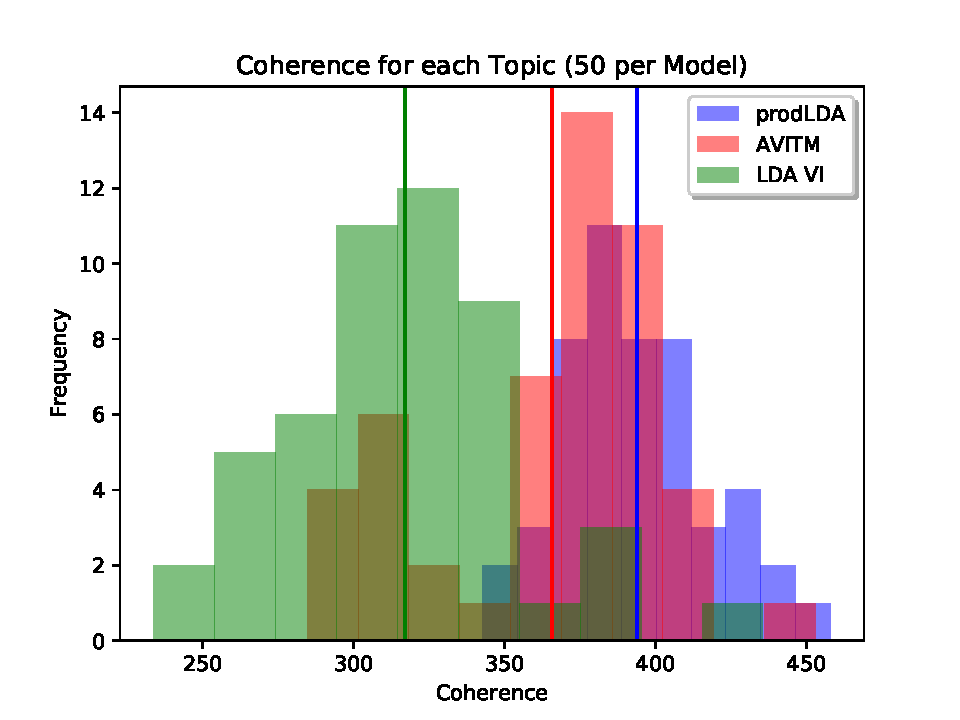
\includegraphics[width=0.8\linewidth]{coherence.pdf}
\end{center}
   \caption{Frequency histogram of topic coherence scores (50 topics total) for each model. 
   The vertical lines represent the mean score for a model's topics.
   Higher coherence scores are more desirable, and indicates intrinsic value of a topic.}
\label{fig:coher}
\end{figure}

\begin{figure*}
\begin{center}
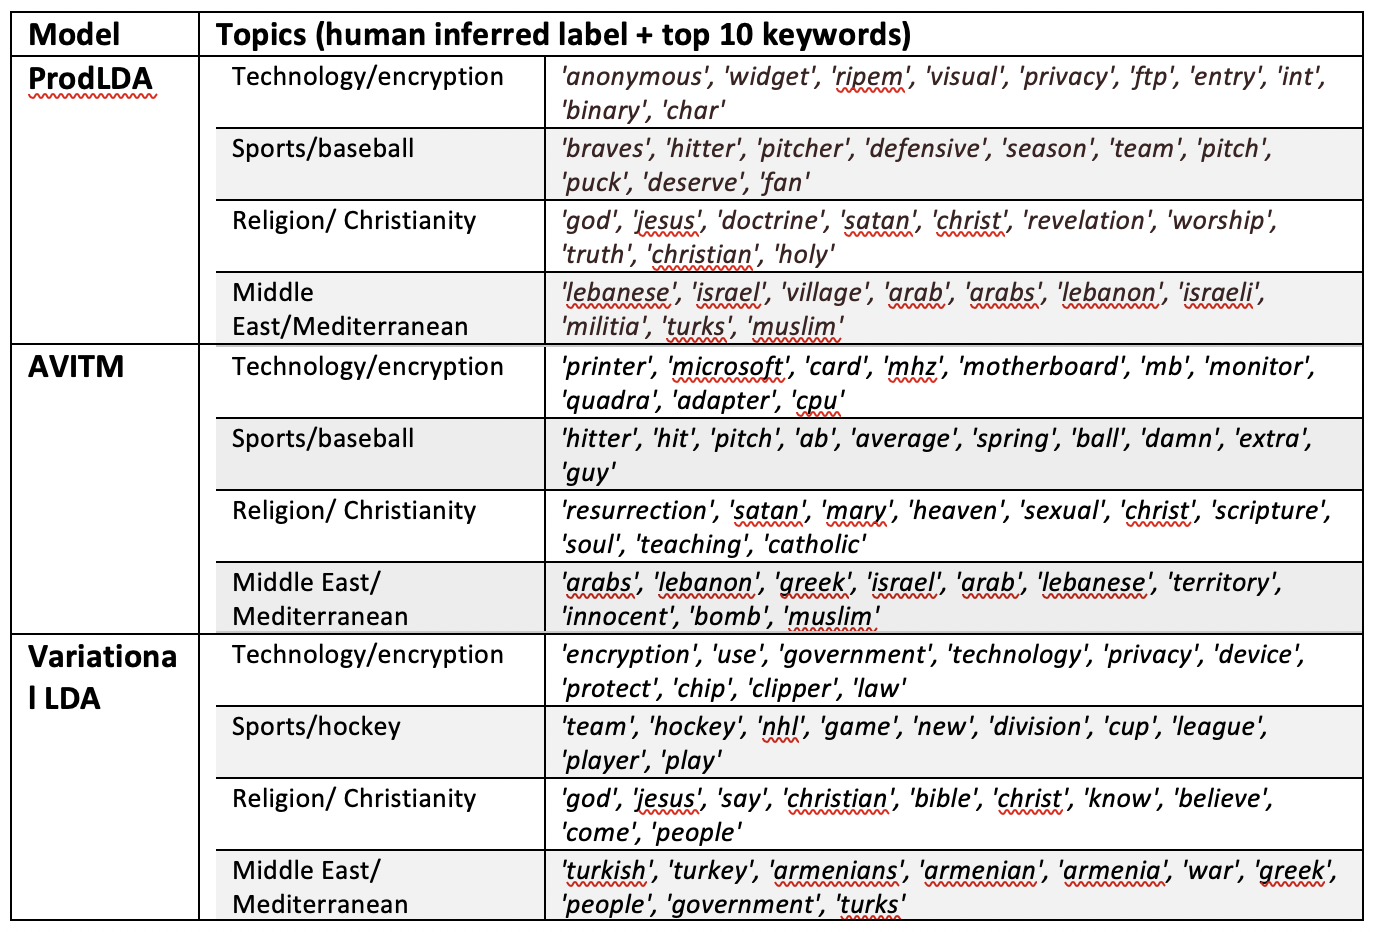
\includegraphics[width=1\linewidth]{qualitative-summary.png}
\end{center}
   \caption{Display of the top 10 keywords for a handful of topics (out of 50 topics total) for each model.}
\label{fig:qual}
\end{figure*}

%-------------------------------------------------------------------------

\section{Detailed Roles}
\noindent
%Fill in the table below for each teammate.
Table \ref{tab:roles} contains the description of each file that I either edited, or wrote from scratch.
\begin{table}\label{tab:roles}
\centering
\begin{tabular}{ |c|c|c| } 
\hline
\textbf{Task} & \textbf{File names} \\
\hline
Run the experiment & run.py  \\ 
Summarize the results of experiment & make\_pls.py  \\ 
Format score code as a module & source/\_\_init\_\_.py \\
Preprocess \& format data & source/data.py \\
Implement AVITM model & source/nvlda.py \\
Implement ProdLDA model & source/prodlda.py \\
Calculate evaluation metrics & source/results.py \\
\hline
\end{tabular}
\caption{List of tasks and their respective files.}
\end{table}

%-------------------------------------------------------------------------
\section{Conclusion}
The objective of this project was to study and replicate the results of the paper ~\cite{srivastava2017autoencoding}.
I was able to achieve the same conclusions as the original paper, as discussed in Section 5.
That is, the models ProdLDA and AVITM find more meaningful topics than LDA VI due to their reparameterization strategy.
This experiment also suggested that topic coherence is a more meaningful quantitative score than perplexity (I.e., model fit) in this setting.
However, my estimated perplexity and topic coherence scores were very different from the original paper.

\paragraph{Challenges.}
The primary challenge in this work was learning the details of implementation for the experiments in ~\cite{srivastava2017autoencoding}.
This information is critical for reproducible experiments.

The hyperparameters are not defined in the paper, along with the approach of the model architecture, described in Section 3.
I learned about them from reading the open-source code of the paper.
I believe that it is very likely that the hyperparameters defined in code are the same values used the paper's experiments.
Yet, I cannot be certain this is true.

Another challenge is that it is not clear \textit{how} or \text{why} many the hyperparamters are selected. 
Varying the values of the hyperparameters used in the experiment may produce different qualitative results for ProdLDA and AVITM.
For instance, it has been shown by ~\cite{wallach2009rethinking} that generative topic models can be sensitive to the prior of the Dirichlet parameter $\theta$.
In addition to prior values, the models may be sensitive to varying the number of predefined topics.

%-------------------------------------------------------------------------
\section{Code Repository}
%Include a link to your GitHub code repository here. The GitHub page should be public and should have a readme file describing briefly what each file does and how to install and run it.
The GitHub repository for this project is \href{https://github.com/kgeyer/cs591-project}{\texttt{https://github.com/kgeyer/cs591-project}}.

%-------------------------------------------------------------------------
{\small
\bibliographystyle{ieee_fullname}
\bibliography{egbib}
}

%-------------------------------------------------------------------------
\end{document}
